% Chapter 1 Introduction
\chapter{ INTRODUCTION} % Main chapter title

\label{chapter1} % For referencing the chapter elsewhere, use \ref{Chapter1} 

%----------------------------------------------------------------------------------------

% Define some commands to keep the formatting separated from the content 
\newcommand{\keyword}[1]{\textbf{#1}}
\newcommand{\tabhead}[1]{\textbf{#1}}
\newcommand{\code}[1]{\texttt{#1}}
\newcommand{\file}[1]{\texttt{\bfseries#1}}
\newcommand{\option}[1]{\texttt{\itshape#1}}

%----------------------------------------------------------------------------------------
Text here

\section{First section}\label{first-section}
Text here; The second section shows how to cite and how to post figures and refer to them.
\subsection{First subsection}
Text here
\subsubsection{First sub subsection}
Text here.
This sub subsection is not included in the Table of Contents and not numbered either.

\section{Figures and Tables}\label{power-sys-def}

\subsection{Figure}
Electrical power system is the holistic order of generation, transmission, distribution and utilization of the electrical energy. Figure \ref{F1-1}, which is modified from \cite{nerc_grid_concept} as per Nepalese context, depicts the generic composition of the power system.
 
\begin{figure}[ht]
    \centering
    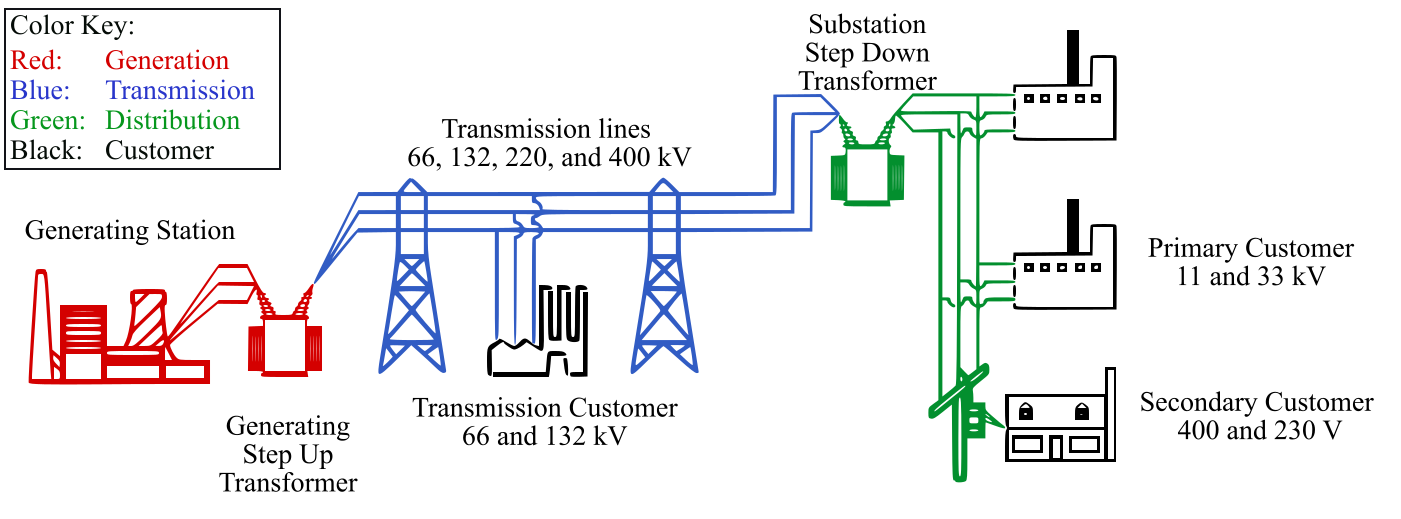
\includegraphics[width=1\textwidth]{Figures/1/Electricity_grid_simple-Nepal.png}
    \caption{Generation, transmission and distribution system of INPS}
    \label{F1-1}
\end{figure}

\subsection{Table}
 Table \ref{T_data_prep} lists out the dataset within each group.

\begin{table}[ht]
\centering
\caption{Prepared datasets for sequential Monte Carlo simulation}
\label{T_data_prep}
\begin{tabular}{|l|l|l|}
\hline
\textbf{SN} & \textbf{Data group} & \textbf{Dataset details} \\ \hline
1           & Feeder data         & Feeder data in OpenDSS   \\ \hline
2 &
  System data &
  \begin{tabular}[c]{@{}l@{}}Line length\\ Distance from service station\\ Circuit breaker information\\ Upstream breaker information\\ Condition monitored component database\end{tabular} \\ \hline
3 &
  Load data &
  \begin{tabular}[c]{@{}l@{}}Load rated kW and multiplier for each hour\\ Load rated kVA and multiplier for  each hour\end{tabular} \\ \hline
4 &
  Rate data &
  \begin{tabular}[c]{@{}l@{}}Failure rates\\ Repair rates\\ Failure rates without detection\\ Condition monitoring rates\\ Condition monitoring fault detection probability\end{tabular} \\ \hline
5 &
  Operational data &
  \begin{tabular}[c]{@{}l@{}}Daytime work hour information\\ Holiday work hour information\\ Weekend work hour information\\ Operational delay information\end{tabular} \\ \hline
6           & Weather data        & Lightning dataset        \\ \hline
\end{tabular}
\end{table}



\section{Code Snippet}
Sample to insert the code snippet from a text file

\begin{adjustbox}{width=\textwidth}
\lstinputlisting[language=Python]{Figures/1/SubXform.txt}
\end{adjustbox}

Another sample. 

\begin{adjustbox}{width=\textwidth}
\lstinputlisting[language=Python]{Figures/1/SubCkt.txt}
\end{adjustbox}

Also check \url{https://carbon.now.sh/} for creating images of code snippets.


\section{Equation and Algorithm}

\subsection{Sample Equation.}
Mathematical derivation of the accuracy level of Monte Carlo simulation is expressed with coefficient of variation in \cite{li1994reliability}. Mathematically, it is expressed in equation \ref{eq_beta}  \cite{li1994reliability}.

\begin{equation}\label{eq_beta}
    \beta = \frac{\sigma}{\mu}
\end{equation}
    \equations{Coefficient of variation of Monte Carlo simulation}
where, $\beta$ is the coefficient of variation, $\sigma$ is the standard deviation and $\mu$ is the mean of the tracking or index variable. The coefficient of variation for energy not served is observed to have the lowest rate of convergence \cite{li1994reliability}. 





\subsection{Sample Algorithm}
Mathematically, time to repair can be expressed as in Equation equation \ref{E5:2} \cite{clements_systemic_2018}.

\begin{equation} \label{E5:2}
    TTR =  N\Big(\frac{1}{\mu}, SD_\mu\Big)
\end{equation}
\equations{Time to repair}
where $\mu$ is the repair rate of the component, N is the normal distribution with Standard Deviation of $SD_\mu$

Clearly, it follows normal distribution and its characteristics are portrayed in Figure \ref{F6_Norm}. Algorithm implemented for time to repair calculation is outlined in Algorithm \ref{alg_ttr}.


  \begin{figure}[htb]
    \centering
    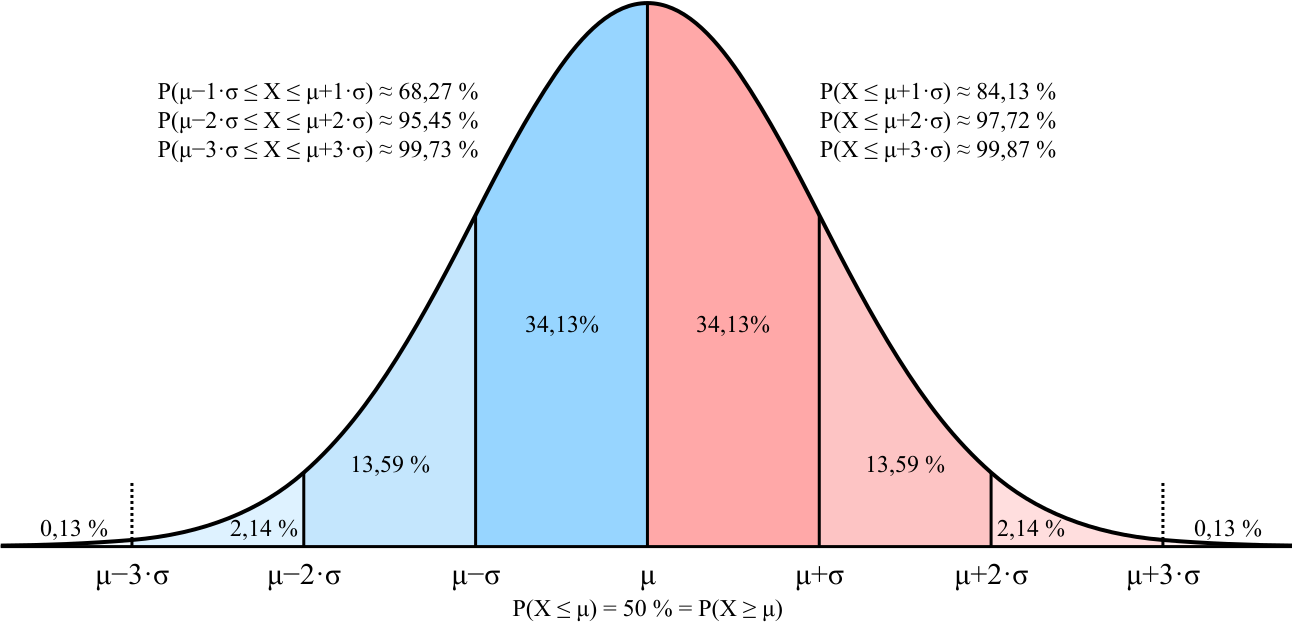
\includegraphics[width=1\textwidth]{Figures/1/Normal_Distribution_Sigma.png}
    \caption{Normal distribution \cite{kowarschick_english_2012}}
    \label{F6_Norm}
\end{figure}
 




\begin{algorithm}[ht]
\SetAlgoLined
% \footnotesize %sano font to reduce the space
\SetKwInOut{Input}{Input} %Input output define gareko tala detail ma lekhna lai
\SetKwInOut{Output}{Output}
\Input{Component i ($C_i$), Repair rate database with repair rate($f_{\mu}$), Normal distribution function $N$}
\Output{time to repair of component i ($ttr_i$)}
%main algorithm begins
  \uIf{Component i repair rate is available}{
    $ttr_i = N\Big(\frac{1}{\mu_i}, SD_{\mu i}\Big) $\;
  }
  \uElseIf{Component i type repair rate is available}{
    $ttr_i = N\Big(\frac{1}{\mu_typei}, SD_{\mu typei}\Big) $\;
  }
  \Else{
    $\mu_i = 20000$ \tcp{have low ttr to avoid error in simulation for exceptions}
    $ttr_i = N\Big(\frac{1}{\mu_i}, SD_{\mu i}\Big)  $\;
  }
 \caption{Determination of time to repair}\label{alg_ttr}
\end{algorithm}






\section{Problem Statement}
Text here
\section{Scope of this thesis}
Text here
\subsection{Objectives of the thesis}
Text here



\section{Thesis Organization}

%%%% The basic idea here is to use \hyperref[label of the link]{Text to be displayed}. Due to unusual requirement of Chapter ONE and Section 1.1 in the template, I have found this way around to be easy (And also within the time frame to write my thesis). It would be great if you could work on some other ideas for this.
The dissertation is organized into seven chapters. This section enlists a brief outline of each chapter and its contents. \begin{itemize}
    \item \hyperref[chapter1]{This chapter} defines the power system in general and introduces the INPS and describes its components. The problem statement is described and followed by specifying the scope, objectives and limitations of the thesis work.
    
    \item Chapter \hyperref[chapter2]{2} provides the literature review on the field of distribution system  reliability analysis, condition monitoring, best practices in the system and prior research works.
    
    \item Chapter \hyperref[chapter3]{3} includes the theoretical aspects of reliability and maintenance. It also briefly describes the software implemented in this study and the sequential Monte Carlo simulation approach.
    
   \item Chapter \hyperref[chapter4]{4} lays the research design and methodology. An overall methodological framework to perform set of tasks to achieve the thesis objective are discussed.
    
    \item Chapter \hyperref[chapter5]{5} discusses the system modeling approach. The cases under study are formulated and the modeling of the system parameters conducted in this study are are described in detail.
    
    \item Chapter \hyperref[chapter6]{6} presents the simulation approach and displays the results of the simulation. Each results also discusses the implications of the results followed by the related discussions.
    
    \item Chapter \hyperref[chapter7]{7} concludes the findings of this study.
    
    \item Appendices provide the supporting information to the thesis. 

\end{itemize}
